\documentclass[10pt]{article}
\usepackage{tikz}
\usetikzlibrary{shapes}

\begin{document}

\textwidth=7in
\textheight=9.5in
\topmargin=-1in
\headheight=0in
\pagestyle{empty}

\begin{center}
{\bf CS165 Database Systems \\
Homework 8 - Indexing \\
Solutions}
\end{center}

\vskip.35in
\noindent Given a B-tree index:

\begin{center}
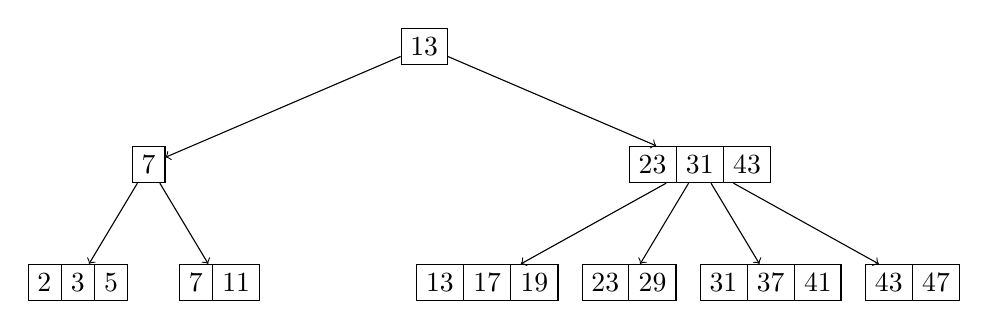
\begin{tikzpicture}
\tikzstyle{bplus}=[
	rectangle split,
	rectangle split horizontal,
	rectangle split ignore empty parts,
	draw ]
\tikzstyle{every node}=[bplus]
\tikzstyle{level 1}=[sibling distance=70mm]
\tikzstyle{level 2}=[sibling distance=18mm]
\node {13} [->]
	child {node {7}
    child {node {2 \nodepart{two} 3 \nodepart{three} 5}}
    child {node {7 \nodepart{two} 11}}
  }
  	child {node {23 \nodepart{two} 31 \nodepart{three} 43}
  	child {node {13 \nodepart{two} 17 \nodepart{three} 19}}
  	child {node {23 \nodepart{two} 29}}
  	child {node {31 \nodepart{two} 37 \nodepart{three} 41}}
  	child {node {43 \nodepart{two} 47}}
  }
;
\end{tikzpicture}
\end{center}

\vskip.10in
\noindent After inserting 15:

\begin{center}
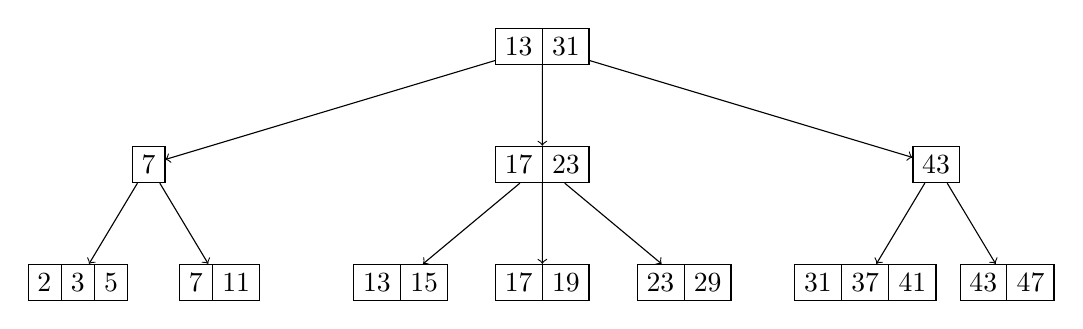
\begin{tikzpicture}
\tikzstyle{bplus}=[
	rectangle split,
	rectangle split horizontal,
	rectangle split ignore empty parts,
	draw ]
\tikzstyle{every node}=[bplus]
\tikzstyle{level 1}=[sibling distance=50mm]
\tikzstyle{level 2}=[sibling distance=18mm]
\node {13 \nodepart{two} 31} [->]
	child {node {7}
    child {node {2 \nodepart{two} 3 \nodepart{three} 5}}
    child {node {7 \nodepart{two} 11}}
  }
  	child {node {17 \nodepart{two} 23}
  	child {node {13 \nodepart{two} 15}}
  	child {node {17 \nodepart{two} 19}}
  	child {node {23 \nodepart{two} 29}}
  }
  	child {node {43}
  	child {node {31 \nodepart{two} 37 \nodepart{three} 41}}
  	child {node {43 \nodepart{two} 47}}
  }
;
\end{tikzpicture}
\end{center}

\vskip.10in
\noindent After inserting 25:

\begin{center}
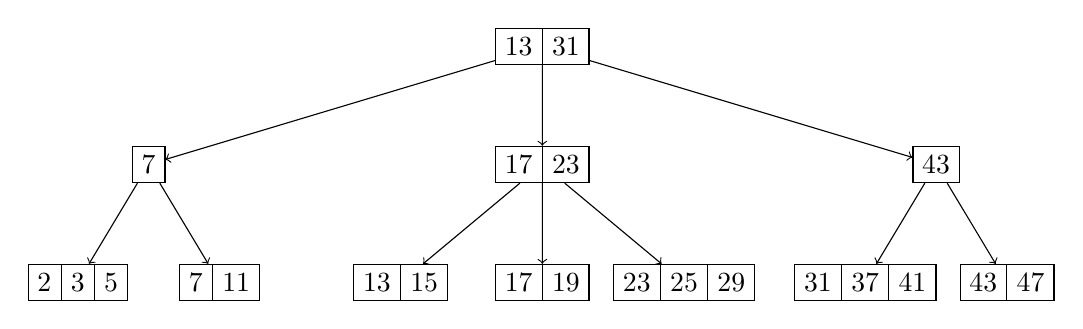
\begin{tikzpicture}
\tikzstyle{bplus}=[
	rectangle split,
	rectangle split horizontal,
	rectangle split ignore empty parts,
	draw ]
\tikzstyle{every node}=[bplus]
\tikzstyle{level 1}=[sibling distance=50mm]
\tikzstyle{level 2}=[sibling distance=18mm]
\node {13 \nodepart{two} 31} [->]
	child {node {7}
    child {node {2 \nodepart{two} 3 \nodepart{three} 5}}
    child {node {7 \nodepart{two} 11}}
  }
  	child {node {17 \nodepart{two} 23}
  	child {node {13 \nodepart{two} 15}}
  	child {node {17 \nodepart{two} 19}}
  	child {node {23 \nodepart{two} 25 \nodepart{three} 29}}
  }
  	child {node {43}
  	child {node {31 \nodepart{two} 37 \nodepart{three} 41}}
  	child {node {43 \nodepart{two} 47}}
  }
;
\end{tikzpicture}
\end{center}

\newpage

\vskip.10in
\noindent After deleting 13:

\begin{center}
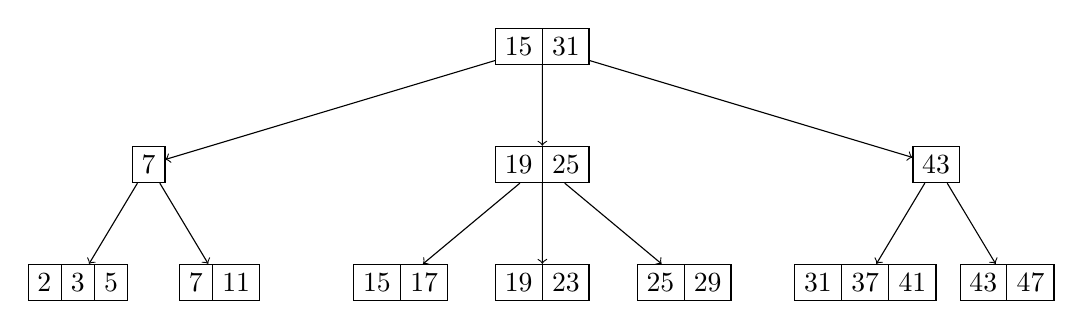
\begin{tikzpicture}
\tikzstyle{bplus}=[
	rectangle split,
	rectangle split horizontal,
	rectangle split ignore empty parts,
	draw ]
\tikzstyle{every node}=[bplus]
\tikzstyle{level 1}=[sibling distance=50mm]
\tikzstyle{level 2}=[sibling distance=18mm]
\node {	15 \nodepart{two} 31} [->]
	child {node {7}
    child {node {2 \nodepart{two} 3 \nodepart{three} 5}}
    child {node {7 \nodepart{two} 11}}
  }
  	child {node {19 \nodepart{two} 25}
  	child {node {15 \nodepart{two} 17}}
  	child {node {19 \nodepart{two} 23}}
  	child {node {25 \nodepart{two} 29}}
  }
  	child {node {43}
  	child {node {31 \nodepart{two} 37 \nodepart{three} 41}}
  	child {node {43 \nodepart{two} 47}}
  }
;
\end{tikzpicture}
\end{center}

\vskip.10in
\noindent After deleting 11:

\begin{center}
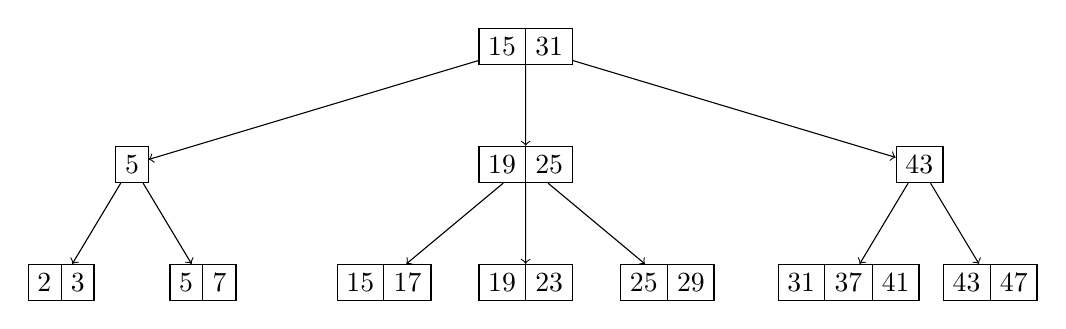
\begin{tikzpicture}
\tikzstyle{bplus}=[
	rectangle split,
	rectangle split horizontal,
	rectangle split ignore empty parts,
	draw ]
\tikzstyle{every node}=[bplus]
\tikzstyle{level 1}=[sibling distance=50mm]
\tikzstyle{level 2}=[sibling distance=18mm]
\node {	15 \nodepart{two} 31} [->]
	child {node {5}
    child {node {2 \nodepart{two} 3}}
    child {node {5 \nodepart{two} 7}}
  }
  	child {node {19 \nodepart{two} 25}
  	child {node {15 \nodepart{two} 17}}
  	child {node {19 \nodepart{two} 23}}
  	child {node {25 \nodepart{two} 29}}
  }
  	child {node {43}
  	child {node {31 \nodepart{two} 37 \nodepart{three} 41}}
  	child {node {43 \nodepart{two} 47}}
  }
;
\end{tikzpicture}
\end{center}

\vskip.10in
\noindent After deleting 7:

\begin{center}
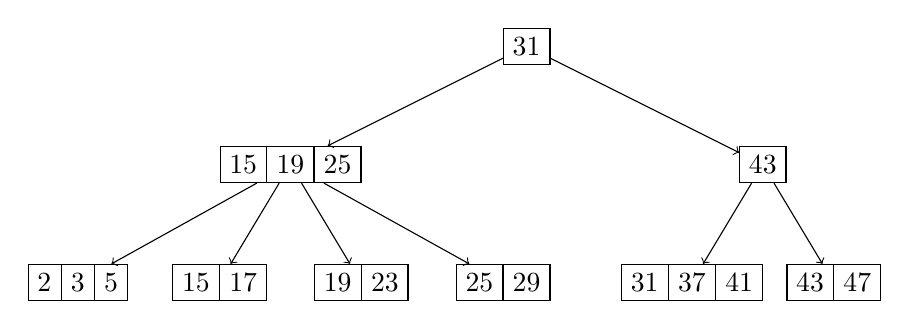
\begin{tikzpicture}
\tikzstyle{bplus}=[
	rectangle split,
	rectangle split horizontal,
	rectangle split ignore empty parts,
	draw ]
\tikzstyle{every node}=[bplus]
\tikzstyle{level 1}=[sibling distance=60mm]
\tikzstyle{level 2}=[sibling distance=18mm]
\node {31} [->]
  	child {node {15 \nodepart{two} 19 \nodepart{three} 25}
  	child {node {2 \nodepart{two} 3 \nodepart{three} 5}}
  	child {node {15 \nodepart{two} 17}}
  	child {node {19 \nodepart{two} 23}}
  	child {node {25 \nodepart{two} 29}}
  }
  	child {node {43}
  	child {node {31 \nodepart{two} 37 \nodepart{three} 41}}
  	child {node {43 \nodepart{two} 47}}
  }
;
\end{tikzpicture}
\end{center}

\end{document}